\problemname{Make Them Meet}

Mila and Laura have been friends online for a long time; they have never met in real life.
Currently, they are both attending the same onsite event, which means that they will surely meet.
However, the hotel where they both are staying is very big and confusing. Therefore, after several days,
they still have not run into each other.

The hotel consists of $N$ rooms, numbered $0$ to $N-1$. Each room has a lamp that can be changed into different colours.
You have found the electrical
service room of the hotel, allowing you to alter the colours of the lamps.
Your goal is to guide Mila and Laura using the lamps to finally make them meet.

The hotel can be represented as a graph with $N$ vertices (the rooms) and $M$ edges (the corridors connecting the rooms).
Mila and Laura
initially start in two different rooms but you do not know which ones. You can make a number
of moves. Each move consists of printing a list of $N$ integers, $c_0, c_1, \ldots, c_{N-1}$, meaning
that the colour of the lamp in room $i$ becomes $c_i$ for every $i = 0,1,\ldots,N-1$. Mila and Laura will then look
at the colour of the lamp in the room they are currently in and walk to a neighbouring room
whose lamp has the same colour. If there is no such neighbouring room, they will stay where
they are.
If there are several such neighbouring rooms, they will choose one arbitrarily.

If Mila and Laura are in the same room or use the same corridor simultaneously at any point during your moves, you have succeeded in making them meet.
You can make at most $20\,000$ moves, but you will
get a higher score if you use fewer moves.

Note that you do not know which rooms Mila and Laura start in or how they walk if they have multiple rooms with the same colour to choose from. \textbf{Your solution must be correct regardless of their starting rooms or how they walk.}

\section*{Input}
The first line contains two integers, $N$ and $M$, the number of rooms and the number of corridors in the hotel respectively.

The following $M$ lines each contain two integers, $u_i$ and $v_i$, meaning that rooms
$u_i$ and $v_i$ are connected by a corridor.

\section*{Output}
Print one line with an integer $K$, the number of moves.

On each of the following $K$ lines, print $N$ integers, $c_0, c_1, \ldots, c_{N-1}$, such that $0\le c_i\le N$ for all $i$. These $K$ lines represent your moves in the chronological order.

\section*{Constraints and Scoring}
\begin{itemize}
\item $2 \leq N \leq 100$.
\item $N-1 \leq M \leq \frac{N(N-1)}{2}$.
\item $0 \leq u_i, v_i \leq N-1$, and $u_{i}\neq v_{i}$.
\item You can reach every room from every other room. Furthermore, there are no corridors going from a room to itself, and there are not multiple corridors between any pair of rooms. 
\item You may use at most $20\,000$ moves (that is, $K\le 20\,000$).
\end{itemize}

Your solution will be tested on a set of test groups, each worth a number of points.
Each test group contains a set of test cases. To get the points for a test group, you need to solve all test cases in the test group.



\begin{tabular}{|c|c|c|}
\hline
Group  &  Max score  &  Limits \\
\hline
  1 & 10 & $M = N-1$, and the corridors are $(0,1), (0,2), (0,3), \ldots, (0,N-1)$. In other words, the graph is a star.   \\
\hline
  2 & 13 & $M = \frac{N(N-1)}{2}$, i.e., there is a corridor between any pair of rooms. In other words, the graph is complete.   \\
\hline
  3 & 11 & $M = N-1$, and the corridors are $(0,1), (1,2), (2,3), \ldots, (N-2,N-1)$. In other words, the graph is a path.   \\
\hline
  4 & 36 & $M = N-1$. In other words, the graph is a tree.   \\
\hline
  5 & 30 & No additional constraints.   \\
\hline
\end{tabular}

For every test group that your program solves correctly, you will receive a score based on the following formula:

\[\text{score} = \left\lfloor S_g \cdot \min\left(1, \frac{2000}{K_g + 1900} + \frac15\right)\right\rfloor ,\]
where $S_g$ is the max score for the test group and $K_g$ is the maximum number of moves that your solution
used for any test case in the test group. This means that in order to get full score, you need to use at most
$600$ moves in all of the test cases. The plot below shows the number of points, as a function of $K_g$.

\begin{figure}
\centering
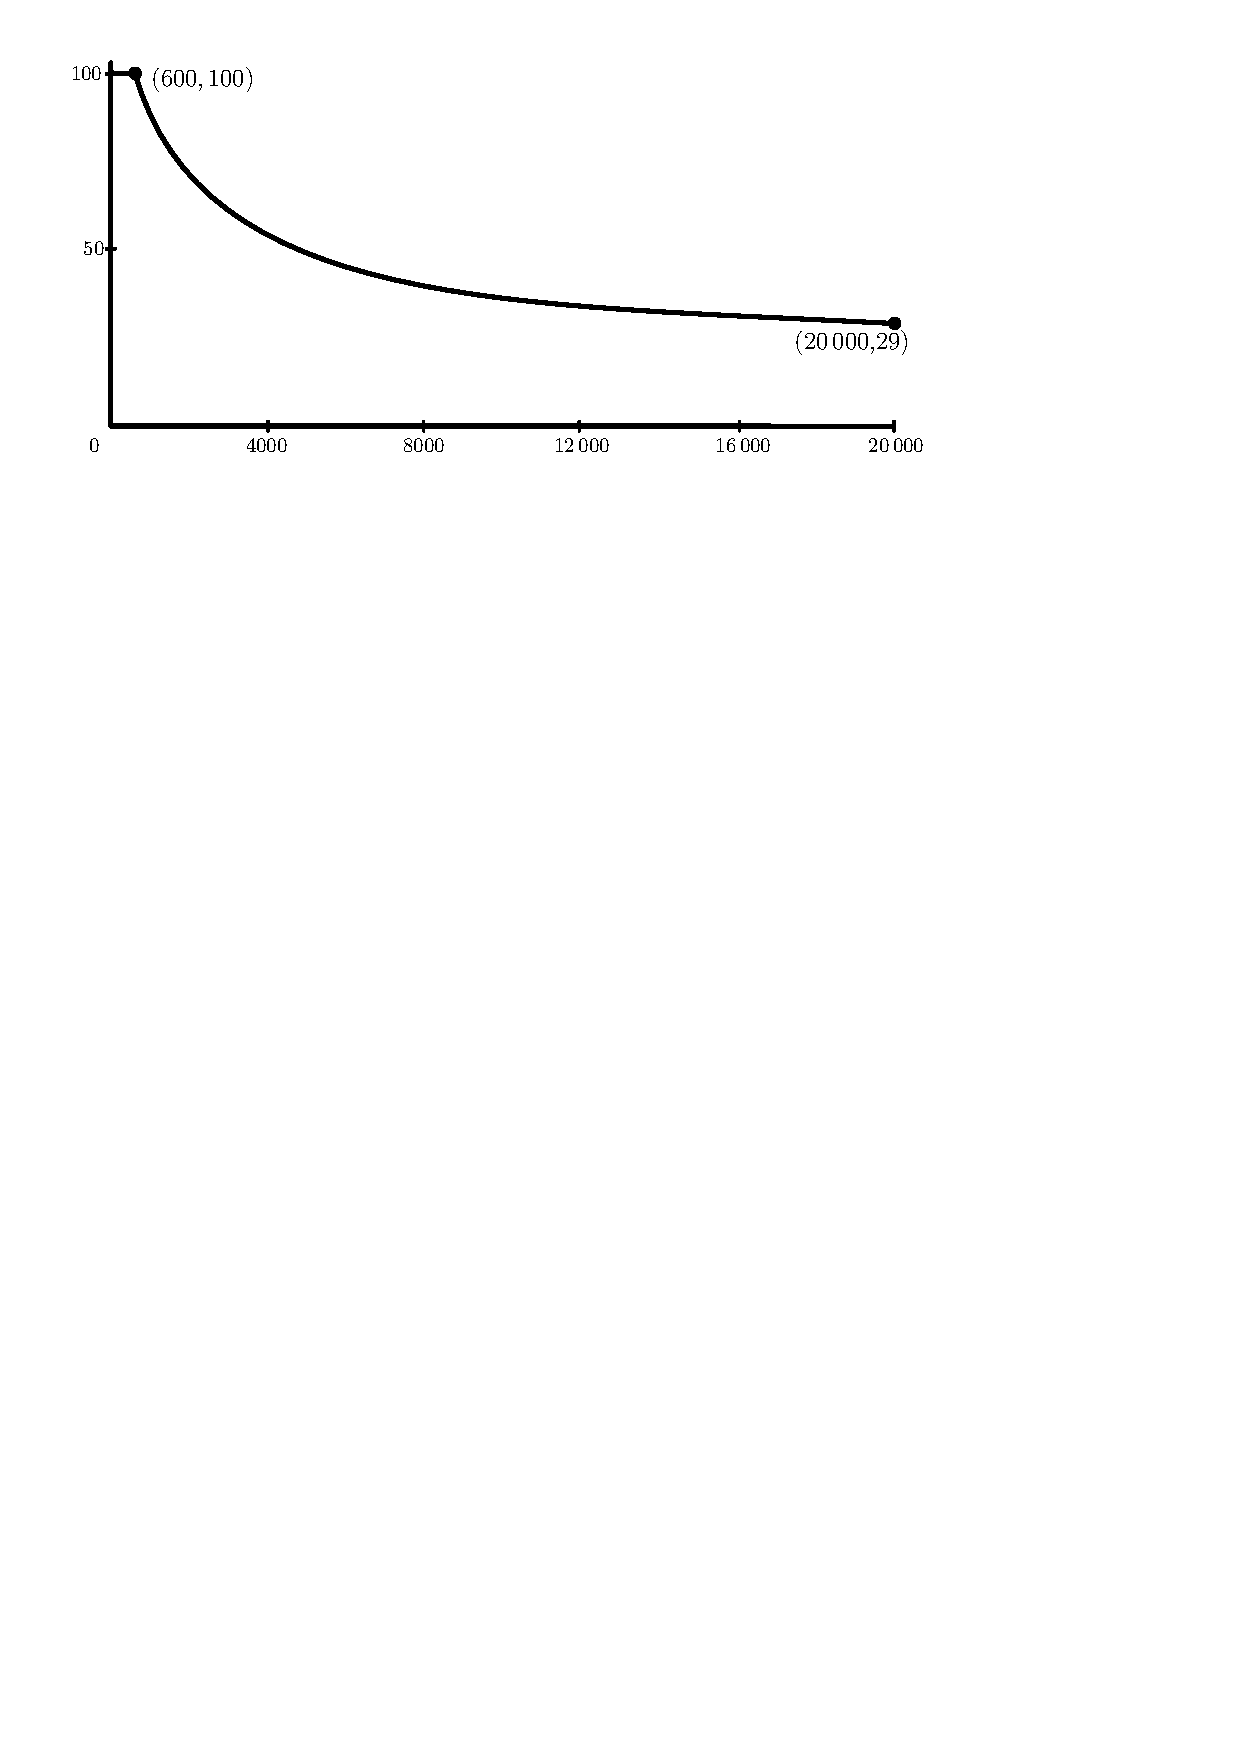
\includegraphics[width=0.95\textwidth]{makethemmeetplot}
\end{figure}

\section*{Example}
The sample case is a path of length $3$, so it could belong to test groups $3$, $4$, or $5$. If
the lamps of the rooms are coloured according to the sample output, then Mila and Laura will always meet.

For example, let us assume that Mila starts in room $0$ and Laura starts in room $1$:

\begin{itemize}
\item First move: Mila must walk to room $1$. If Laura walks to room $0$, then they will
  meet in the corridor between $0$ and $1$. Let us say that Laura walks to room $2$ instead.
\item Second move: Mila walks back to room $0$ and Laura stays in room $2$.
\item Third move: Mila walks to room $1$ again and Laura stays in room $2$.
\item Fourth move: Mila walks to room $2$ and Laura walks to room $1$. Thus,
  they will meet on the corridor between rooms $1$ and $2$.
\item Fifth move: Mila and Laura swaps places and meet again
  (but it does not matter since they already met).
\end{itemize}

The figure below shows the first four moves of the sample.
\begin{figure}
\centering
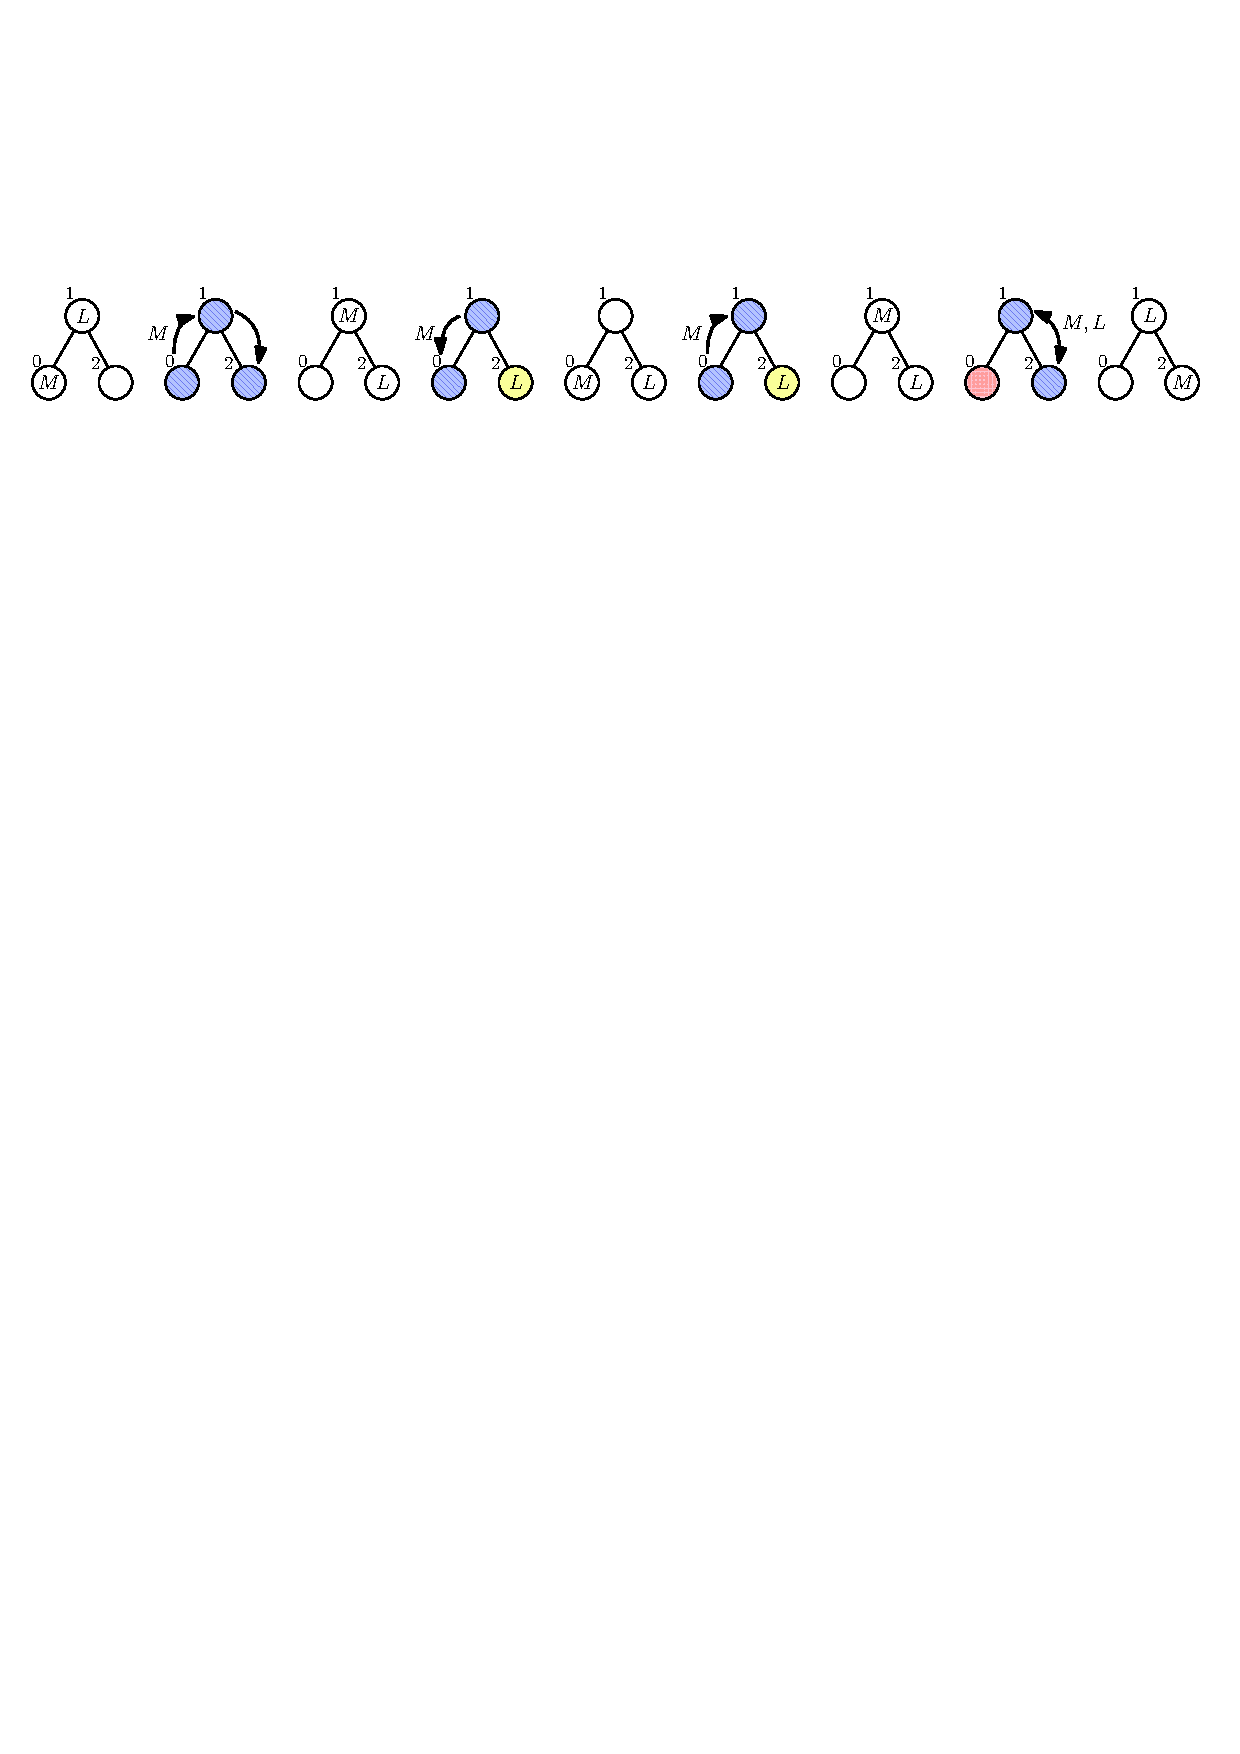
\includegraphics[width=0.95\textwidth]{sample}
\end{figure}

Note that this was only the case where the friends start in the rooms $0$ and $1$.
One can verify that the same sequence of moves ensures that they will meet, regardless of where they start and how they walk.


